\section{Coupling}

\subsection{Introduction}

One of the primary goals of the ESMF project is to increase interoperability
across a range of Earth system modeling components.  As described in 
Section~\ref{sec:scope}, initially these 
components will be large scale, such as land models, ocean models, 
data assimilation systems and diagnostics packages.  ESMF coupling 
services will facilitate component 
interoperability and efficient inter-component communication.  As the 
framework evolves, we plan to utilize coupling services for smaller-scale 
tasks within model components, such as the transformation of data between the 
physics and dynamics in a spectral atmospheric model, or the creation 
of nested higher resolution regions within a coarser grid.  The ability to 
couple components at varying scales both flexibly and efficiently requires
careful design and implementation.  In this section, we 
explain the classes involved in ESMF coupled applications, their 
relationships, and the sequence of actions given a number of different 
coupling configurations.  These include a single executable configuration in 
which application components execute sequentially, and a multiple executable
configuration in which model components execute concurrently.

\subsection{Classes and Scoping}

An ESMF coupled application involves an application component
({\tt ESMF\_App})
containing two or more gridded components ({\tt ESMF\_GComp}s) that require an 
inter-component data exchange, and one or more coupling 
components ({\tt ESMF\_Coupler}).

There are restrictions on how objects within an application may be scoped
on a parallel platform.  The application component must be instantiated on 
any decomposition elements or DEs ({\tt ESMF\_DE}s) on which other components
within the application are defined.  This is true whether the 
application contains a single executable or multiple 
executables.  There is only one application component defined for any
application; it initially allocates resources and tracks application-wide 
information.  

A coupler component must be instantiated on any DEs on which components
it will couple are defined.  This is consistent with an architectural
model in which inter-process communication is handled internal to 
a component (see Section~\ref{sec:strategies}).  It is possible for
some portions of the functionality of a component to be restricted to
a subset of the DEs over which the component is defined.  For example, 
it might be computationally efficient for the computation of interpolation
weight to occur on a set of DEs which is 

A gridded component may exist across all DEs in the application.  When 
a set of gridded  components and a coupler all reside on the same set of 
DEs and are contained within an application running as a single 
executable we have an SPMD, sequential execution model.  

Within an application, a gridded component may also reside on 
a subset of DEs.  These may wholly coincide with, be wholly 
contained within or wholly contain another component.  Multiple gridded 
components or couplers may be defined as separate executables.  A typical 
MPMD, concurrent execution configuration is one in which gridded components 
and a coupler are defined on separate DEs running simultaneously as multiple 
executables.

It is possible for ESMF applications to be a combination of the SPMD, 
sequential 
execution model and the MPMD, concurrent execution model.  We might have,
for example, atmosphere and land components defined on the same set of 
DEs and running as one executable, and ocean and sea ice 
components defined on a separate set of DEs and running as 
another executable, with a separate coupler executable running on yet 
another set.  The application component must be defined
on all sets of DEs.

\subsection{Flow of Control and Data}

Gridded components have few responsibilities with respect to coupling
to other components.  They do not need to keep track of the data needed
by other components, compute fluxes, perform grid transformations, or 
perform inter-component transfers of data.  They {\bf are} responsible for 
providing a description of all of the fields and data they
can export to other components, and for similarly providing a description 
of the fields they must import in order to run.  These descriptions are
embodied in the {\tt ESMF\_State} class, and the kind of data that they 
represent is identified by the {\tt type} attribute of that class, which can
have an {\tt ESMF\_IMPORT} or {\tt ESMF\_EXPORT} value.  In addition to 
providing an import state, gridded components are required to check that 
initial or imported data is valid and complete.

The coupler component produces a specification of the sequence of 
transforms that are 
necessary to effect communication between components, both scientific and 
computational.  This specification includes the transforms to be
called, on which DEs they should take place, any sequencing restrictions 
on the transforms, and what data is to be acted on.  For example, the
coupler may specify that transformations occur on either the data sending 
or receiving end (or both), that data be sent directly between components,
or that data be sent to the coupler for intermediate processing before 
it is sent to its destination.  The coupler is not responsible for 
transferring data between components or for managing synchronization; 
these tasks are handled by the application.  

The application component manages the sequencing and synchronization of
components, and applies the transforms specified by the coupler.  The 
configurations that it can support are subject to the restrictions
determined by the coupler.

\subsection{Examples}

In our first set of examples, involving just two components, we'll call 
the instance of the application {\tt app}, the gridded components {\tt atm} 
and {\tt ocn}, and the coupler {\tt coupler}.

\subsection{Object Model}

The hierarchy of classes in ESMF is shown in the following UML diagrams.  

\subsection{Components}

The top level object in the system is a Component object.
Types of components are shown in the diagram below:

\scalebox{0.70}{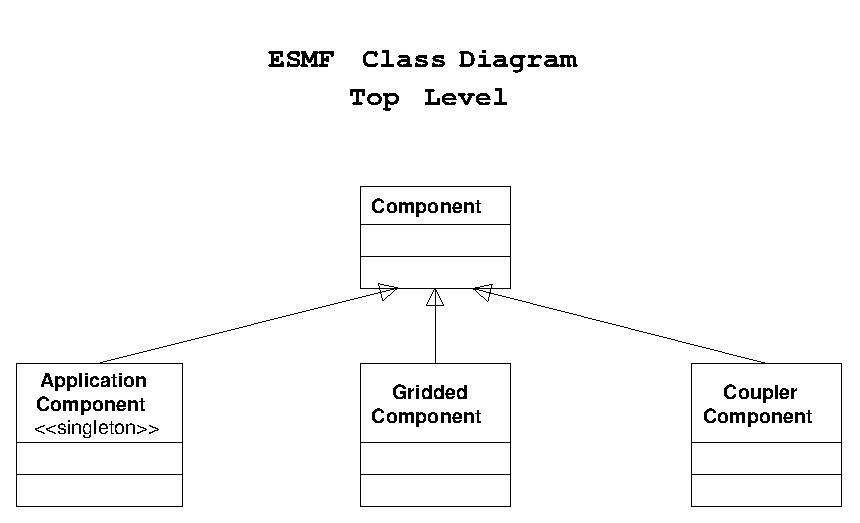
\includegraphics{ESMFTopClassDiagram.eps}}

Detailed descriptions of these objects are:

\subsubsection{Component (ESMF\_Comp)} 
\begin{description}
\item [Description] A Component is a functionally related computational entity that represents 
a large system.  
% \item [Function]  ...
\end{description}

\subsubsection{Application (ESMF\_App)}
\begin{description} 
\item [Description] We define an Application (ESMF\_App) as a special kind of Component 
that is itself composed of a set of sub-Components that interact to form a complete scientific
application.  
\item [Function] The ESMF\_App class is responsible for managing those functions that relate 
to an entire scientific application running under ESMF.  The ESMF\_App initialize method 
must be called at the start of any user application operating under the framework, and
the ESMF\_App finalize method at its end.  At initialization the Application allocates and 
configures any resources needed to run the framework.  The Application also specifies whether 
the system will be brokered using the Registry or not.  The ESMF\_App class can be queried 
for information such as an experiment name, model name, run type (ESMF\_INIT, 
ESMF\_BRANCH, etc.), and for an overall Status.  It can also be queried for
information on any Component that it includes, including its Name, Map, and
Status.
\end{description}

\subsubsection{Coupler Component (ESMF\_Coupler)}
\begin{description}
\item [Description] A Coupler is a specialized type of Component that encompasses all the 
functionality needed to communicate data between two or more Components. 
\item [Function] A Coupler must have methods to register new Components, to negotiate
which Components need to exchange data, with optional Transformations of data, and to
mediate the actual data exchange.
\end{description}

\subsubsection{Gridded Component (ESMF\_GComp)}
\label{sec:griddedcomponent} 
\begin{description}
\item [Description] A Gridded Component is a specialized type of Component that is associated
with computational data and the grid on which it is located.
\item [Function] The GComp class is an abstraction to unify the grid and data carrying
objects in the system: the Grid class, the Field class, and the Bundle class.
<< what common Methods are at this level?? >>
\end{description}

\subsubsection{Transform (ESMF\_XForm)} 
\begin{description}
\item [Description] A Transform takes one or more physical quantities defined using one set 
of units or representation and translates them as needed to a different set of units or 
representation, for example, potential temperature to temperature.  Transform objects 
are specialized by the application developer.
\item [Function] The Transform class is an abstraction introduced for the
purpose of standardizing high-level coupling interfaces.  It may be overloaded
to take sets of individual Fields or Bundles.  Methods may include a
separate initialization and run. 
\item [Note] << this object was in the text here, but doesn't
exist in the corresponding diagram.  which one needs to be fixed?? >>
\end{description}






